\documentclass[17pt]{beamer}
%\documentclass[handout]{beamer} %Makes Handouts
\usetheme{Singapore} %Gray with fade at top
\useoutertheme[subsection=false]{miniframes} %Supppress subsection in header
\useinnertheme{rectangles} %Itemize/Enumerate boxes
\usecolortheme{seagull} %Color theme
\usecolortheme{rose} %Inner color theme

\definecolor{light-gray}{gray}{0.75}
\definecolor{dark-gray}{gray}{0.55}
\setbeamercolor{item}{fg=light-gray}
\setbeamercolor{enumerate item}{fg=dark-gray}

\setbeamertemplate{navigation symbols}{}
\setbeamertemplate{mini frames}{}
%\setbeamercovered{dynamics}
\setbeamerfont*{title}{size=\Large,series=\bfseries}
\setbeamerfont{footnote}{size=\tiny}

%\setbeameroption{notes on second screen} %Dual-Screen Notes
%\setbeameroption{show only notes} %Notes Output

\setbeamertemplate{frametitle}{\vspace{.5em}\bfseries\insertframetitle}
\newcommand{\heading}[1]{\noindent \textbf{#1}\\ \vspace{1em}}
\newcommand{\questions}{\frame{{\large Questions?}}}

\usepackage{bbding,color,multirow,times,ccaption,tabularx,graphicx,verbatim,booktabs}
\usepackage{colortbl} %Table overlays
\usepackage[english]{babel}
\usepackage[latin1]{inputenc}
\usepackage[T1]{fontenc}
\usepackage{lmodern}
\usepackage{alltt}

\usepackage{tikz}
\usetikzlibrary{shapes,arrows,decorations.pathreplacing,calc}


\author[]{Thomas J. Leeper}
\institute{
  Government Department\\London School of Economics and Political Science
}


\title{Session II\\Examples and Paradigms}

\date[]{}

\begin{document}

\frame{\titlepage}

\frame{\tableofcontents}


\section[Hypotheses > Design]{Translating Hypotheses into Designs}
\frame{\tableofcontents[currentsection,currentsubsection,subsubsectionstyle=hide]}


\frame{

\frametitle{From Theory to Design}

\begin{itemize}\itemsep1em
\item From theory, we derive testable hypotheses
\begin{itemize}
\item Hypotheses are expectations about differences in outcomes across levels of a putatively causal variable
\end{itemize}
\item Hypothesis must be testable by an SATE ($H_0=0$)
\item Manipulations are developed to create variation in that causal variable
\end{itemize}

}


\frame{

\frametitle{{\normalsize Example: News Framing}}

\small

\begin{itemize}
\item Theory: Presentation of news affects opinion
\item Hypotheses:
	\begin{itemize}\footnotesize
	\item News emphasizing free speech increases support for a hate group rally
	\item News emphasizing public safety decreases support for a hate group rally
	\end{itemize}
\item Manipulation:
	\begin{itemize}\footnotesize
	\item Control group: no information
	\item Free speech group: article emphasizing rights
	\item Public safety group: article emphasizing safety
	\end{itemize}
\end{itemize}

}




\frame{

\frametitle{{\normalsize Example: Partisan Identity}}

\small

\begin{itemize}
\item Theory: Strength of partisan identity affects tendency to accept party position
\item Hypotheses:
	\begin{itemize}\small
	\item Strong partisans are more likely to accept their party's position on an issue
	\end{itemize}
\item Manipulation:
	\begin{itemize}\small
	\item Control group: no manipulation
	\item ``Univalent'' condition
	\item ``Ambivalent'' condition
	\end{itemize}
\end{itemize}

}


\frame[label=ambivalentpartisan]{

\frametitle{\textbf{\only<1>{Univalent}\only<2>{Ambivalent}}}

These days, Democrats and Republicans differ from one another considerably. The two groups seem to be growing further and further apart, not only in terms of their opinions but also their lifestyles. Earlier in the survey, you said you tend to identify as a \textit{Democrat/ Republican}. Please take a few minutes to think about what you like about \textit{Democrats/ Republicans} compared to the \textit{Republicans/ Democrats}. Think of 2 to 3 things you especially like best about \textbf{\only<1>{your party}\only<2>{the other party}}. Then think of 2 to 3 things you especially dislike about \textbf{\only<2>{your party}\only<1>{the other party}}. Now please write those thoughts in the space below.

}



\frame{

\frametitle{Treatments Test Hypotheses!}

\begin{itemize}\itemsep1em
\item<2-> Experimental ``factors'' are expressions of hypotheses as randomized groups
\item<3-> What stimulus each group receives depends on hypotheses
\item<4-> Three ways hypotheses lead to stimuli:
	\begin{itemize}
	\item presence/absence
	\item levels/doses
	\item qualitative variations
	\end{itemize}
\end{itemize}

}


\frame{

\frametitle{{\normalsize Ex.: Presence/Absence}}

\small

\begin{itemize}\itemsep0.5em
\item Theory: Negative campaigning reduces support for the party described negatively.
\item Hypothesis: Exposure to a negative advertisement criticizing a party reduces support for that party.
\item Manipulation:
	\begin{itemize}\small 
	\item Control group receives no advertisement. 
	\item Treatment group watches a video containing a negative ad describing a party.
	\end{itemize}
\end{itemize}

}


\frame{

\frametitle{{\normalsize Ex.: Levels/doses}}

\small

\begin{itemize}\itemsep-0.2em
\item Theory: Negative campaigning reduces support for the party described negatively.
\item Hypothesis: Exposure to higher levels of negative advertising criticizing a party reduces support for that party.
\item Manipulation:
	\begin{itemize}\footnotesize
	\item Control group receives no advertisement. 
	\item Treatment group 1 watches a video containing 1 negative ad describing a party.
	\item Treatment group 2 watches a video containing 2 negative ads describing a party.
	\item Treatment group 3 watches a video containing 3 negative ads describing a party.
	\item etc.
	\end{itemize}
\end{itemize}

}


\frame{

\frametitle{{\normalsize Ex.: Qualitative variation}}

\small

\begin{itemize}
\item Theory: Negative campaigning reduces support for the party described negatively.
\item Hypothesis: Exposure to a negative advertisement criticizing a party reduces support for that party, while a positive advertisement has no effect.
\item Manipulation:
	\begin{itemize}\footnotesize
	\item Control group receives no advertisement. 
	\item Negative treatment group watches a video containing a negative ad describing a party.
	\item Positive treatment group watches a video containing a positive ad describing a party.
	\end{itemize}
\end{itemize}

}

\questions


\section{Assessing Quality}
\frame{\tableofcontents[currentsection,currentsubsection,subsubsectionstyle=hide]}

\frame{

\frametitle{Activity!}

\begin{itemize}\itemsep0.5em
\item How do we know if an experiment is any good?
\item Talk with a partner for about 3 minutes
\item Try to develop some criteria that allow you to evaluate ``what makes for a good experiment?'' 
\end{itemize}

}


\frame{

\frametitle{Some possible criteria}

\small

\begin{itemize}\itemsep-0.2em
\item Significant results
\item Face validity
\item Coherent for respondents
\item Non-obvious to respondents
\item Simple
\item Indirect/unobtrusive
\item Validated by prior work
\item Innovative/creative
\item \dots
\end{itemize}

}


\frame{

\begin{quote}\large
The best criterion for evaluating the quality of an experiment is whether it manipulated the intended independent variable and controlled everything else by design.
\end{quote}
\onslide<2->{\small\hspace{5em} --Thomas J. Leeper (5 February 2018)}

}

\frame{

\frametitle{How do we know we manipulated what we think we manipulated?}

\small

\begin{itemize}
\item<2-> Outcomes are affected consistent with theory
\item<3-> Before the study using \textit{pilot testing} (or \emph{pretesting})
\item<4-> During the study, using \emph{manipulation checks}
\item<5-> During the study, using \emph{placebos}
\item<6-> During the study, using \textit{non-equivalent outcomes}
\end{itemize}
}

\frame{

\frametitle{I. Outcomes Affected}

\begin{itemize}\itemsep0.5em
\item Follows a circular logic!
\item Doesn't tell us anything if we hypothesize null effects
\end{itemize}

}


\frame{

\frametitle{II. Pilot Testing}

\small

\begin{itemize}\itemsep0.2em
\item Goal: establish construct validity of manipulation
\item Assess whether a set of possible manipulations affect a measure of the \textit{independent} variable
\item<2-> Example:
	\begin{itemize}
	\item Goal: Manipulate the ``strength'' of an argument
	\item Write several arguments
	\item Ask pilot test respondents to report how strong each one was
	\end{itemize}
\end{itemize}

}

\frame{

\frametitle{III. Manipulation Checks}

\small

\begin{itemize}\itemsep0.2em
\item Manipulation checks are items added post-treatment, post-outcome that assess whether the \textit{independent} variable was affected by treatment
\item We typically talk about manipulations as directly setting the value of $X$, but in practice we are typically manipulating something \textit{that we think} strongly modifies $X$
\item<2-> Example: information manipulations aim to modify knowledge or beliefs, but are necessarily imperfect at doing so
\end{itemize}

}

\frame{

\frametitle{\normalsize Manipulation check example\footnote{Leeper \& Slothuus. n.d. ``Can Citizens Be Framed?'' Available from: \url{http://thomasleeper.com/research.html}.}}

\begin{enumerate}
\item Treatment 1: Supply Information
\item Manipulation check 1: measure beliefs
\item Treatment 2: Prime a set of considerations
\item Outcome: Measure opinion
\item Manipulation check 2: measure dimension salience
\end{enumerate}

}


\frame{

\frametitle{{\normalsize Some Best Practices}}


\begin{itemize}\itemsep0.5em
\item<2-> Manipulation checks should be innocuous
	\begin{itemize}
	\item Shouldn't modify independent variable
	\item Shouldn't modify outcome variable
	\end{itemize}
\item<3-> Generally, measure post-outcome
\item<4-> Measure both what you wanted to manipulate \textit{and} what you didn't want to manipulate
	\begin{itemize}
	\item Most treatments are \textit{compound}!
	\end{itemize}
\end{itemize}

}

\frame{

\frametitle{IV. Placebos}

\begin{itemize}\itemsep0.5em
\item Include an experimental condition that \textit{does not} manipulate the variable of interest (but might affect the outcome)
\item<2-> Example:
	\begin{itemize}
	\item Study whether risk-related arguments about climate change increase support for a climate change policy
	\item Placebo condition: control article with risk-related arguments about non-environmental issue (e.g., terrorism)
	\end{itemize}
\end{itemize}

}

\frame{

\frametitle{V. Non-equivalent outcomes}

\small

\begin{itemize}\itemsep0.5em
\item Measures an outcome that \textit{should not} be affected by independent variable
\item<2-> Example:
	\begin{itemize}
	\item Assess effect of some treatment on attitudes toward group A
	\item Focal outcome: attitudes toward group A
	\item Non-equivalent outcome: attitudes toward group B
	\end{itemize}
\end{itemize}

}


\frame{

\frametitle{{\normalsize Aside: Demand Characteristics}}

\small

\begin{itemize}\itemsep0.5em
\item ``Demand characteristics'' are features of experiments that (unintentionally) imply the purpose of the study and thereby change respondents' behavior (to be consistent with theory)
\item<2-> Implications:
	\begin{itemize}\footnotesize
	\item Design experimental treatments that are non-obvious
	\item Do not disclose the purpose of the study up front\footnote{But, consider the ethics of not doing so (more Friday)}
	\end{itemize}
\end{itemize}

}




\section[Examples]{Common Paradigms and Examples}
\frame{\tableofcontents[currentsection,currentsubsection,subsubsectionstyle=hide]}


\frame{

\frametitle{Question Wording Designs}

\begin{itemize}\itemsep1em
\item Simplest paradigm for presence/absence or qualitative variation
\item Manipulation operationalizes this by asking two different questions
\item Outcome is the answer to the question
\item Example: Schuldt et al. ```Global Warming' or `Climate Change'? Whether the Planet is Warming Depends on Question Wording.''
\end{itemize}

}

\frame{

\small

You may have heard about the idea that the world's temperature may have been \textbf{\only<1>{going up}\only<2>{changing}} over the past 100 years, a phenomenon sometimes called \textbf{\only<1>{global warming}\only<2>{climate change}}. What is your personal opinion regarding whether or not this has been happening?
	\begin{itemize}\itemsep-0.25em\footnotesize
	\item Definitely has not been happening
	\item Probably has not been happening
	\item Unsure, but leaning toward it has not been happening
	\item Not sure either way
	\item Unsure, but leaning toward it has been happening
	\item Probably has been happening
	\item Definitely has been happening
	\end{itemize}
}


\frame{

\frametitle{{\normalsize Another framing example\footnote{Singer \& Couper. 2014. ``The Effect of Question Wording on Attitudes toward Prenatal Testing and Abortion.'' \textit{Public Opinion Quarterly} 78(3): 751--760.}}}

\footnotesize

Today, tests are being developed that make it possible to detect serious genetic defects \textbf{\only<1>{before a baby is born}\only<2>{in the fetus during pregnancy}}. But so far, it is impossible either to treat or to correct most of them. If (you/your partner) were pregnant, would you want (her) to have a test to find out if the \textbf{\only<1>{baby}\only<2>{fetus}} has any serious genetic defects? (Yes/No)\\

\vspace{0.5em}

Suppose a test shows the \textbf{\only<1>{baby}\only<2>{fetus}} has a serious genetic defect. Would you, yourself, want (your partner) to have an abortion if a test shows the \textbf{\only<1>{baby}\only<2>{fetus}} has a serious genetic defect? (Yes/No)

}


\frame{

\frametitle{{\normalsize Another framing example\footnote{Bobo \& Johnson. 2004. ``A Taste for Punishment: Black and White Americans' Views on the Death Penalty and the War on Drugs.'' Du Bois Review 1(1): 151--180.}}}

\only<2>{Blacks are about 12\% of the U.S. population, but they were half of the homicide offenders last year. }Do you favor or oppose the death penalty for persons convicted of murder?

}

\frame{

\frametitle{{\normalsize Another framing example\footnote{Haider-Markel \& Joslyn. 2001. ``Gun Policy, Opinion, Tragedy, and Blame Attribution: The Conditional Influence of Issue Frames.'' \textit{Journal of Politics} 63(2): 520--543.}}}

\only<1>{Concealed handgun laws have recently received national attention. Some people have argued that law-abiding citizens have the right to protect themselves.}\only<2>{Concealed handgun laws have recently received national attention. Some people have argued that laws allowing citizens to carry concealed handguns threaten public safety because they would allow almost anyone to carry a gun almost anywhere, even onto school grounds.} What do you think about concealed handgun laws?

}





\frame{

\frametitle{{\normalsize Question Order Designs}}

\small

\begin{itemize}
\item Manipulation of pre-outcome questionnaire
\item<2-> Example:
	\begin{itemize}
	\item Goal: assess influence of value salience on support for a policy
	\item Manipulate by asking different questions:
		\begin{itemize}
		\item Battery of 5 ``rights'' questions, or
		\item Battery of 5 ``life'' questions
		\end{itemize}
	\item Measure support for legalized abortion
	\end{itemize}
\item<3-> If answers to manipulated questions matter, can measure rest post-outcome
\end{itemize}

}

\frame{
	\frametitle{{\normalsize Ex. Question-as-treatment\footnote{Transue. 2007. ``Identity Salience, Identity Acceptance, and Racial Policy Attitudes: {American} National Identity as a Uniting Force.'' \textit{American Journal of Political Science} 51(1): 78--91.}}}
	

\begin{itemize}
\item \only<1,3>{How close do you feel to your ethnic or racial group?}\only<2,4>{How close do you feel to other Americans?}
\item \only<1-2>{Some people have said that taxes need to be raised to take care of pressing national needs. How willing would you be to have your taxes raised to improve education in public schools?}\only<3-4>{Some people have said that taxes need to be raised to take care of pressing national needs. How willing would you be to have your taxes raised to improve educational opportunities for minorities?}
\end{itemize}
	
}


\frame{

\frametitle{{\normalsize Ex.: Knowledge and Political Interest}}

\footnotesize

\begin{enumerate}
\item Do you happen to remember anything special that your U.S. Representative has done for your district or for the people in your district while he has been in Congress?
\item Is there any legislative bill that has come up in the House of Representatives, on which you remember how your congressman has voted in the last couple of years?
\item Now, some people seem to follow what's going on in government and public affairs most of the time, whether there's an election going on or not. Others aren't that interested. Would you say that you follow what's going on in government and public affairs most of the time, some of the time, only now and then, or hardly at all?
\end{enumerate}

}

\frame{

\frametitle{{\normalsize Ex.: Knowledge and Political Interest}}

\footnotesize

\begin{enumerate}
\item Now, some people seem to follow what's going on in government and public affairs most of the time, whether there's an election going on or not. Others aren't that interested. Would you say that you follow what's going on in government and public affairs most of the time, some of the time, only now and then, or hardly at all?
\item Do you happen to remember anything special that your U.S. Representative has done for your district or for the people in your district while he has been in Congress?
\item Is there any legislative bill that has come up in the House of Representatives, on which you remember how your congressman has voted in the last couple of years?
\end{enumerate}

}


\frame{

\frametitle{{\normalsize An Instructional Manipulation\footnote{Sturgis, Allum \& Smith. 2008. ``An Experiment on the Measurement of Political Knowledge in Surveys.'' \textit{Public Opinion Quarterly} 72(1): 90--102.}}}

\small

For the next few questions, I am going to read out some statements, and for each one, please tell me if it is true or false. If you don't know, \only<1>{just say so and we will skip to the next one}\only<2>{please just give me your best guess}.

\begin{enumerate}\footnotesize
\item Britain's electoral system is based on proportional representation.
\item MPs from different parties are on parliamentary committees.
\item The Conservatives are opposed to the ratification of a constitution for the European Union.
\end{enumerate}

}


\frame{

\frametitle{{\normalsize An Instructional Manipulation + \footnote{Prior \& Lupia. 2008. ``Money, Time, and Political Knowledge: Distinguishing Quick Recall and Political Learning Skills.'' \textit{American journal of Political Science} 52(1): 169--183.}}}

\small

\only<1>{In the next part of this study, you will be asked 14 questions about politics, public policy, and economics. Many people don't know the answers to these questions, but it is helpful for us if you answer, even if you're not sure what the correct answer is. We encourage you to take a guess on every question. At the end of this study, you will see a summary of how many questions you answered correctly.}\only<2>{We will pay you for answering questions correctly.
You will earn \$1 for every correct answer you give. So, if you answer 3 of the 14 questions correctly, you will earn \$3. If you answer 7 of the 14 questions correctly, you will earn \$7. The more questions you answer correctly, the more you will earn.}

}



\frame{

\frametitle{Vignettes}

\begin{itemize}
\item A ``vignette'' is a short text describing a situation
\item Vignettes are probably the most common survey experimental paradigm, after question wording designs
\item Take many forms and increasingly encompass non-textual stimuli
\item Basically limited to web-based mode
\end{itemize}

}

\frame{

\frametitle{A classic vignette\footnote{Gilens, M. 1996. ```Race coding' and white opposition to welfare. \textit{American Political Science Review} 90(3): 593--604.}}

\small

Now think about a \textbf{(black/white)} woman in her early thirties. She is a high school \textbf{(graduate/drop out)} with a ten-year-old child, and she has been on welfare for the past year.

\begin{itemize}\footnotesize
\item How likely is it that she will have more children in order to get a bigger welfare check? (1 = Very likely, \dots, 7 = Not at all likely)
\item How likely do you think it is that she will really try hard to find a job in the next year? (1 = Very likely, \dots, 7 = Not at all likely)
\end{itemize}
}


\frame{

\frametitle{{\normalsize Newer vignette\footnote{Banerjee et al. 2012. ``Are Poor Voters Indifferent to Whether Elected Leaders are Criminal or Corrupt? A Vignette Experiment in Rural India.'' Working paper.}}}

\footnotesize

Imagine that you were living in a village in another district in Uttar Pradesh and that you were voting for candidates in \textbf{(village/state/national)} election. Here are the two candidates who are running against each other: The first candidate is named \textbf{(caste name)} and is running as the \textbf{(BJP/SP/BSP)} party candidate. \textbf{(Corrupt/criminality allegation)}. His opponent is named \textbf{(caste name)} and is running as the \textbf{(BJP/SP/BSP)} party candidate. \textbf{(Opposite corrupt/criminality allegation)}. From this information, please indicate which candidate you would vote for in the \textbf{(village/state/national)} election. 

}



\frame{

\frametitle{{\normalsize Longer vignette example\footnote{Merolla \& Zechmeister. 2013. ``Evaluating Political Leaders in Times of Terror and Economic Threat: The Conditioning Influence of Politician Partisanship.'' \textit{Journal of Politics} 75(3): 599--712.}}}

\begin{center}
\includegraphics<1>[width=.85\textwidth]{images/merollazechmeister1}
\includegraphics<2>[width=.85\textwidth]{images/merollazechmeister2}
\end{center}

}


\frame{

\frametitle{{\large Some vignette considerations}}

\begin{itemize}\small
\item<2-> Comparability across conditions
	\begin{itemize}
	\item Length
	\item Readability
	\end{itemize}
\item<3-> Language proficiency
\item<4-> Length
	\begin{itemize}\small
	\item Timers
	\item Forced exposure
	\item Mouse trackers
	\end{itemize}
\item<5-> Devices
	\begin{itemize}\small
	\item Browser-specificity
	\item Device sizes (e.g., mobile)
	\end{itemize}
\end{itemize}

}


\frame{

\begin{center}
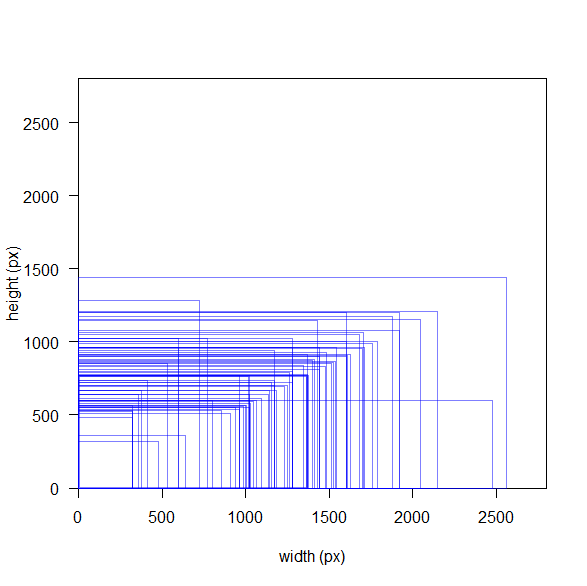
\includegraphics[height=\textheight]{images/devicesizes.png}
\end{center}
}


\frame{

\frametitle{Non-textual Manipulations}

\small

\begin{itemize}\itemsep0.5em
\item Images can work well
\item Standalone or embedded in a text or question
\item<2-> Examples
	\begin{itemize}\footnotesize
	\item<2-> Kalmoe \& Gross\footnote{``Cueing Patriotism, Prejudice, and Partisanship in the Age of Obama: Experimental Tests of U.S. Flag Imagery Effects in Presidential Elections.'' \textit{Political Psychology}: in press.} measure impact of patriotic cues on candidate support by showing images of candidates with and without flags
	\item<3-> Subliminal primes possible, depending on software
	\item<4-> Lots of recent examples of facial manipulation
	\end{itemize}

\end{itemize}

}

\frame{

\frametitle{Example\footnote{Iyengar et al. 2010. ``Do Explicit Racial Cues Influence Candidate Preference? The Case of Skin Complexion in the 2008 Campaign.'' Working paper.}}

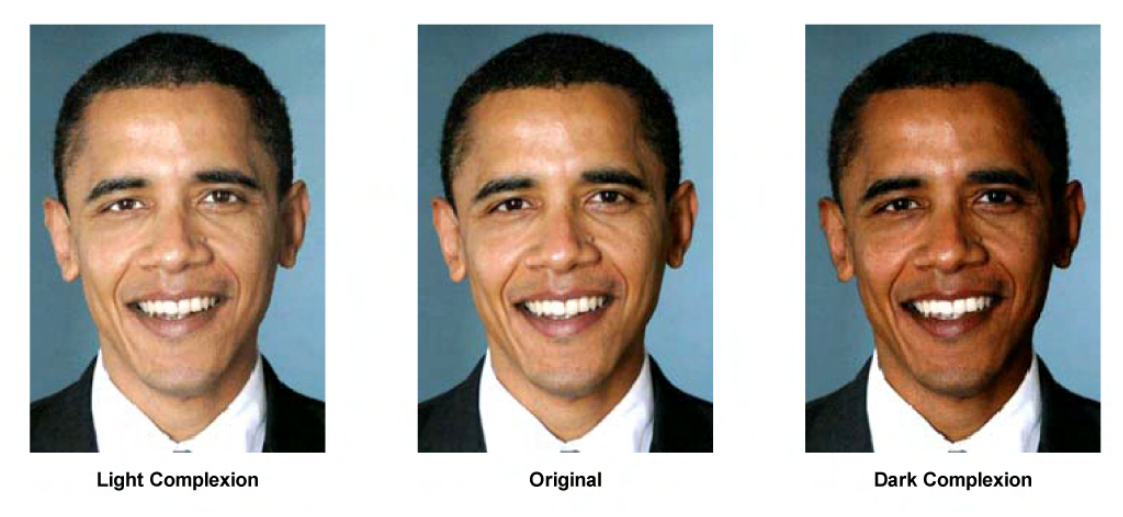
\includegraphics[width=\textwidth]{images/IyengarMessingBailenson}

}

\frame{

\frametitle{{\normalsize Example\footnote{Laustsen \& Petersen. 2016. ``Winning Faces vary by Ideology.'' \textit{Political Communication} 33(2): 188--211.}}}

\begin{center}
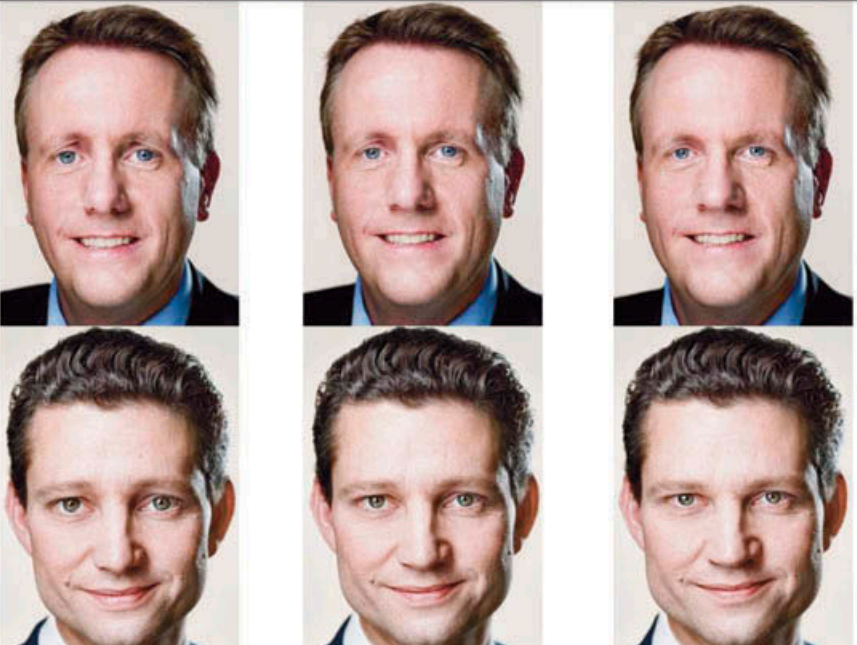
\includegraphics[width=\textwidth, trim={0cm 0cm 0cm 9cm}, clip]{images/laustsen}
\end{center}
}

\frame{
\frametitle{{\normalsize Example\footnote{Bailenson et al. 2006. ``Transformed Facial Similarity as a Political Cue: A Preliminary Investigation.'' \textit{Political Psychology} 27(3): 373--385.}}}

\begin{center}
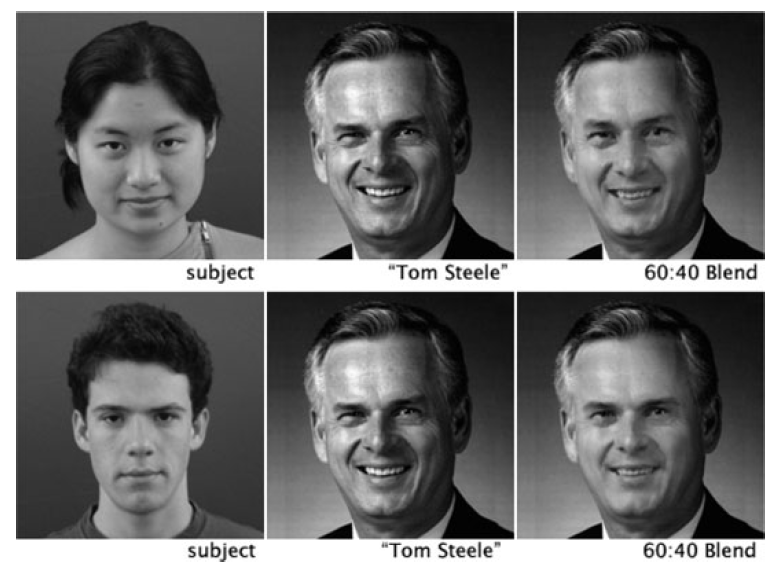
\includegraphics[width=\textwidth, trim={0cm 7.7cm 0cm 0cm}, clip]{images/BailensonGarlandIyengar}
\end{center}
}




\frame{

\frametitle{{\normalsize Audio \& Video manipulations}}

\small

\begin{itemize}\itemsep-0.2em
\item Problematic for same reasons as long texts
\item<2-> Best practices
	\begin{itemize}\footnotesize
	\item Keep it short
	\item Have the video play automatically
	\item Disallow survey progression
	\item Control and validate
	\end{itemize}
\item<3->Examples
	\begin{itemize}
	\item Television Advertisements\footnote{Vavreck. 2007 ``The Exaggerated Effects of Advertising on Turnout: The Dangers of Self-Reports.'' \textit{Quarterly Journal of Political Science} 2: 325--343.} 
	\item News Programs\footnote{Mutz. 2007. ``Effects of `In-Your-Face' Television Discourse on Perceptions of a Legitimate Opposition.'' \textit{American Political Science Review} 101(4): 621--635.}
	\end{itemize}	
\end{itemize}

}




\frame{
\frametitle{``Task'' Designs}

\begin{itemize}\itemsep0.5em
\item Task designs ask respondents to perform a task
\item Often developed for laboratory settings
\item<2-> Most common example: writing something
\item<3-> Can be problematic:
	\begin{itemize}
	\item Time-intensive
	\item Invites drop-off
	\item Compliance problems
	\end{itemize}
\end{itemize}

}


\againframe{ambivalentpartisan}



\questions


\section[More Designs]{More Advanced Designs}
\frame{\tableofcontents[currentsection,currentsubsection,subsubsectionstyle=hide]}

\frame{

\frametitle{Beyond Simple Designs}

\begin{enumerate}\itemsep1em
\item Factorial designs
\item Sensitive question designs
\item Conjoint designs
\item Multi-component designs
	\begin{itemize}
	\item Over-time measurement/randomization
	\item Field--survey combinations
	\end{itemize}
\end{enumerate}
}



\frame{

\frametitle{Sensitive Item Designs}

\begin{itemize}\itemsep1em
\item Randomization can be used to measure something

\item List experiments
	\begin{itemize}
	\item Randomly present lists of items of varying length
	\item Difference in count of items supported is prevalence of sensitive attitude/behavior
	\end{itemize}

\item Randomized response
	\begin{itemize}
	\item Present a sensitive question
	\item Use a randomization device to dictate whether the respondent answers the sensitive question or something else
	\end{itemize}
\end{itemize}
}

\frame{

\frametitle{{\normalsize List Experiments \footnote{Kuklinski et al. 1997. ``Racial Prejudice and Attitudes Toward Affirmative Action.'' \textit{American Journal of Political Science} 41(2): 402--419.}}}

\small

Now I'm going to read you three things that sometimes make people angry or upset. After I read all three, just tell me \textit{how many} of them upset you. I don't want to know which ones. just \textit{how many}.

\footnotesize

\begin{enumerate}
\item the federal government increasing the tax on gasoline
\item professional athletes getting million-dollar salaries
\item large corporations polluting the environment
\item<2-> \textbf{a black family moving in next door}
\end{enumerate}

}


\frame{

\frametitle{Randomized Response\footnote{Blair, Imai, and Zhou. 2015. ``Design and Analysis of the Randomized Response Technique.'' \textit{JASA} 110(511): 1304--19.}}

\begin{itemize}\itemsep1em
\item Example:

{\footnotesize
Here is a bag; in it there are stones from the game `Go,' some colored black and others white. Please take one stone out, and see by yourself what color it is, black or white. Don't let me know whether it is black or white, but be sure you know which it is.\\

If you take a black one, answer the question: ``Have you ever had an induced abortion?''\\

If you take a white one, answer the question: ``Were you born in the lunar year of the horse?'
}

\item Considerations:
	\begin{itemize}
	\item Can use any randomization device
	\item Can be cognitively complex
	\end{itemize}
\end{itemize}




}



\frame{}





% CONJOINTS
\frame{

\frametitle{Conjoint Analysis}

\begin{itemize}\itemsep1em
\item Surveys measure \textit{stated} preferences
\item Conjoint analysis involves measuring \textit{revealed} preferences based upon a series of forced-choice decisions

	\begin{itemize}
	\item Present respondents with pairs of ``profiles'' containing many \textit{features}
	\item Force respondents to choose which of the two they prefer
	\end{itemize}

\item Estimate \textit{relative} importance of features of each profile

\item Randomization of profile features gives differences in preferences across attributes a causal meaning 

\end{itemize}

}


\frame{

\frametitle{Advantages/Disadvantages}

\begin{itemize}\itemsep1em
\item Advantages

\begin{itemize}
\item Reduces ``cheap talk'' results
\item Lower social desirability biases
\item Mimics real-world decisions
\item Revealed preferences are causally interpretable
\end{itemize}

\item Disadvantages

\begin{itemize}
\item More cognitively complex for respondents than traditional polling
\item No straightforward ``\% support'' statistics
\end{itemize}

\end{itemize}

}

\frame{

\frametitle{Structure of Conjoints}

\begin{itemize}\itemsep1em
\item Three examples:
	\begin{enumerate}
	\item Policy preference on Brexit negotiations
	\item Choice of BBC Director General
	\item Choice of a lodger
	\end{enumerate}

\item All are binary, forced-choice designs 

\item Analysis is all focused on AMCEs or subgroup AMCEs

	\begin{itemize}
	\item Estimated using OLS dummy variable regression
	\end{itemize}
\end{itemize}

}


\frame{

\frametitle{{\normalsize Conjoint 1: Brexit Negotiations}}

\begin{center}
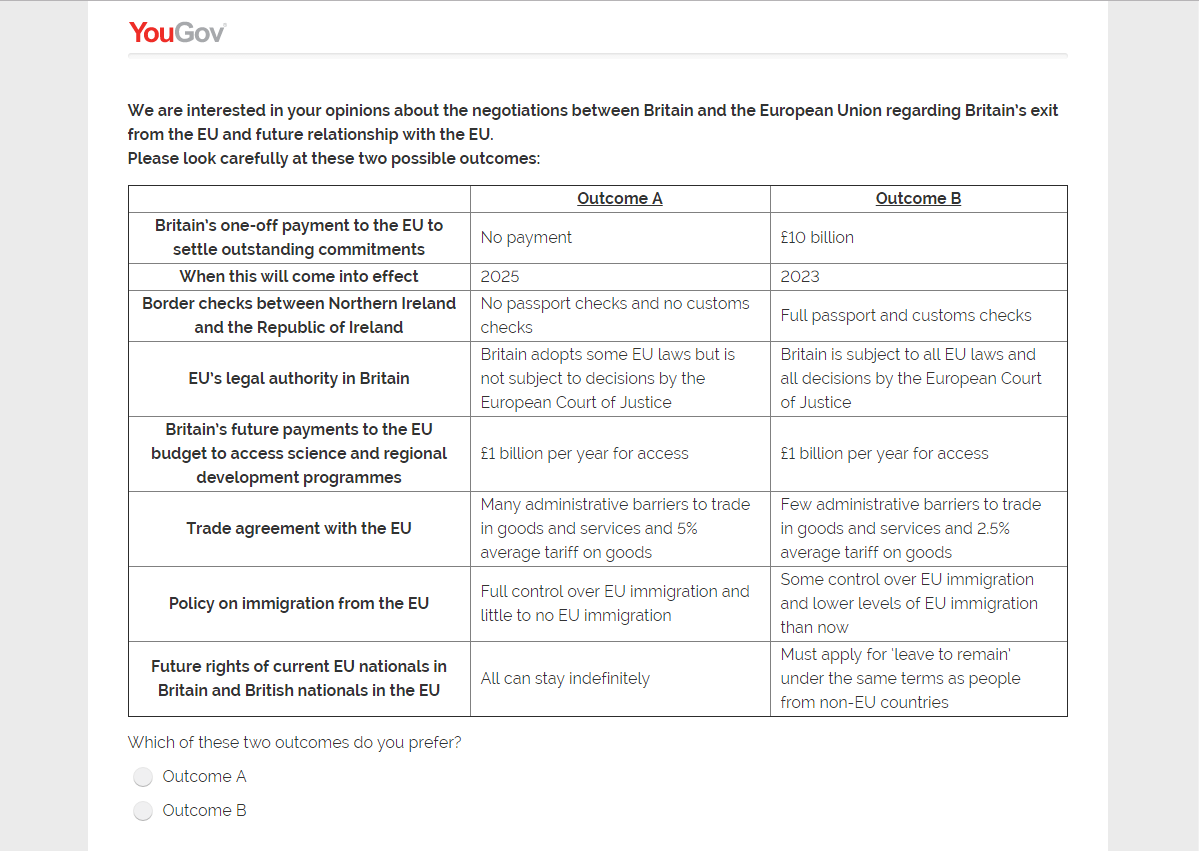
\includegraphics[height=.9\textheight]{images/brexit-conjoint-screenshot}
\end{center}
}


\frame{

\frametitle{{\normalsize Conjoint 2: BBC Director}}

\small
Imagine that you are deciding who to appoint as the next Director General of the BBC. You have received the following information about two applicants and need to make a decision between them.\\

\vspace{1em}

\begin{columns}\footnotesize
\begin{column}{.5\textwidth}
 - Tom\\
 - 68 years old\\
 - Has worked 21 years for the BBC\\
 - Has a degree from the University of Oxford\\
 - Didn't vote at the 2017 election\\
 - Voted Remain in the EU referendum\\
 - Former lawyer
\end{column}
\begin{column}{.5\textwidth}
 - Claire\\
 - 35 years old\\
 - Has never worked for the BBC\\
 - Has a PhD from the University of Exeter\\
 - Voted Conservative at the 2017 election\\
 - Didn't vote in the EU referendum\\
 - Former television producer
\end{column}
\end{columns}

\vspace{1em}

Which of the two applicants would you prefer as the next Director General of the BBC?

}


\frame{

\frametitle{{\normalsize Conjoint 3: Lodger}}

\small
Imagine that you have a spare room that you want to rent out to a lodger. You have received the following information about two possible lodgers and need to make a decision between them.\\

\vspace{1em}

\begin{columns}\footnotesize
\begin{column}{.5\textwidth}
 - James\\
 - 19 years old\\
 - Full-time student\\
 - Helps out at the local Anglican church\\
 - Didn't vote at the 2017 election\\
 - Voted Remain in the EU referendum\\
 - Likes watching rugby
\end{column}
\begin{column}{.5\textwidth}
 - Becky\\
 - 35 years old\\
 - Works for a private company\\
 - Volunteers at an Oxfam shop\\
 - Voted Conservative at the 2017 election\\
 - Didn't vote in the EU referendum\\
 - Likes playing videogames
\end{column}
\end{columns}

\vspace{1em}

Which of the two lodgers would you prefer? 

}



\frame{
\frametitle{AMCEs}

Statistic of interest is the \textit{average marginal component effect} (AMCE), which is the causal effect of each level of each feature on support for an overall profile.

\vspace{1em}

We can estimate this using (dummy variable) OLS, assuming:

\begin{itemize}
\item Full randomization of attributes and randomized pairing of profiles
\item Even presentation of levels w/in features
\item No profile ordering effects
\end{itemize}

}

\frame{
\begin{center}
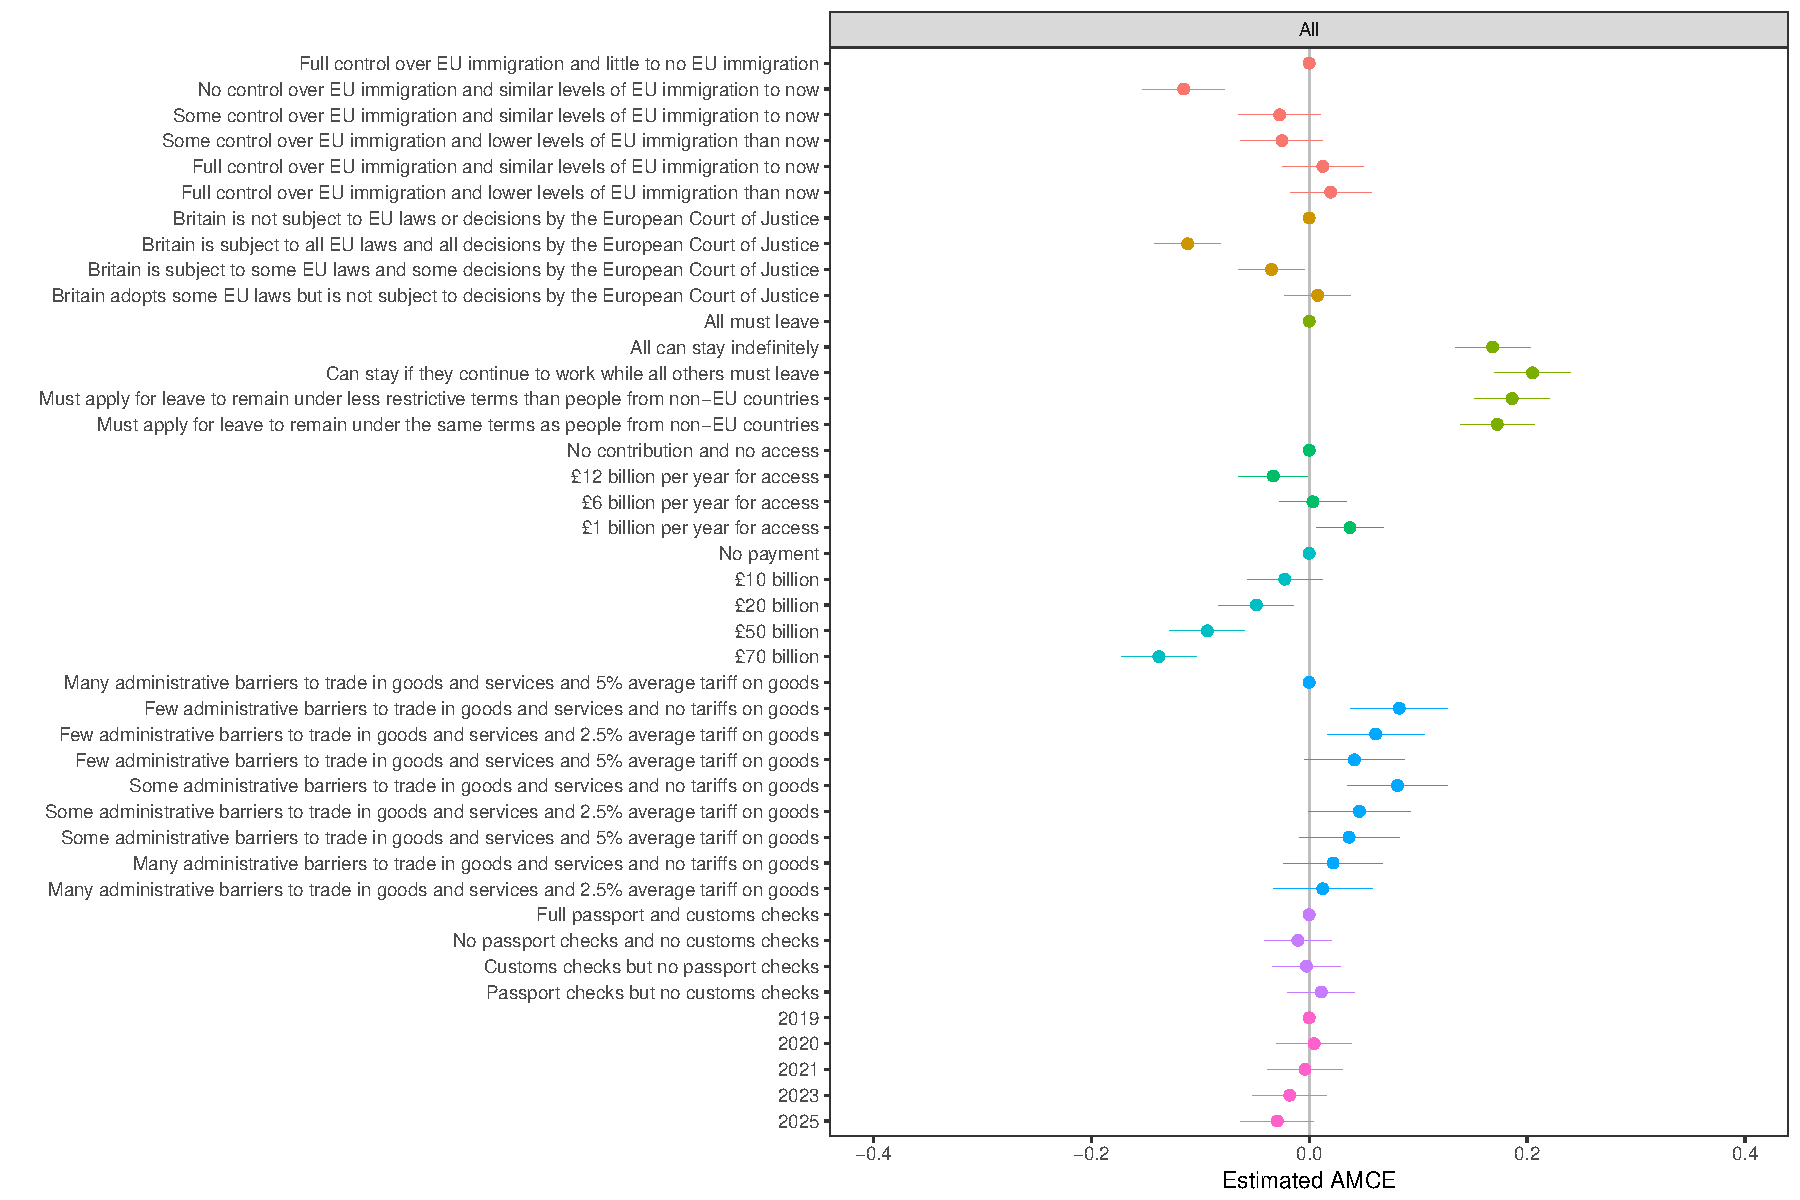
\includegraphics[width=\textwidth]{images/brexit-conjoint}
\end{center}
}

\frame{
\begin{center}
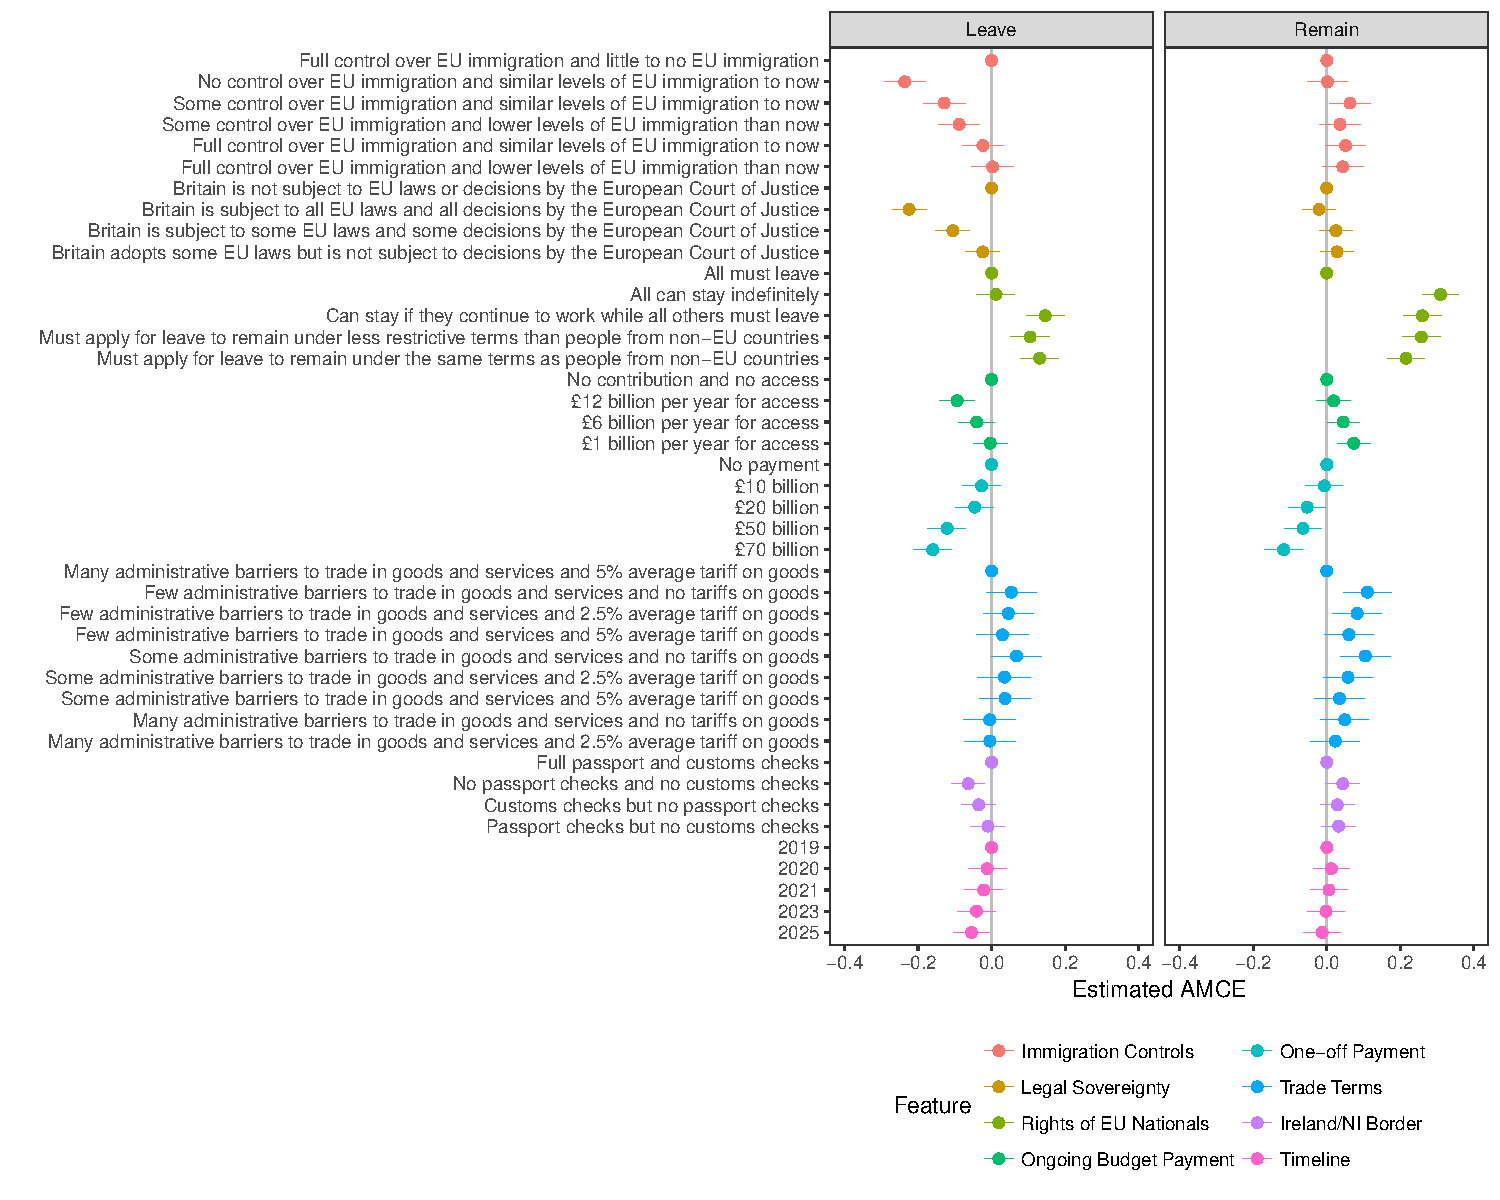
\includegraphics[height=\textheight]{images/brexit-conjoint-split}
\end{center}
}

\frame{
\begin{center}
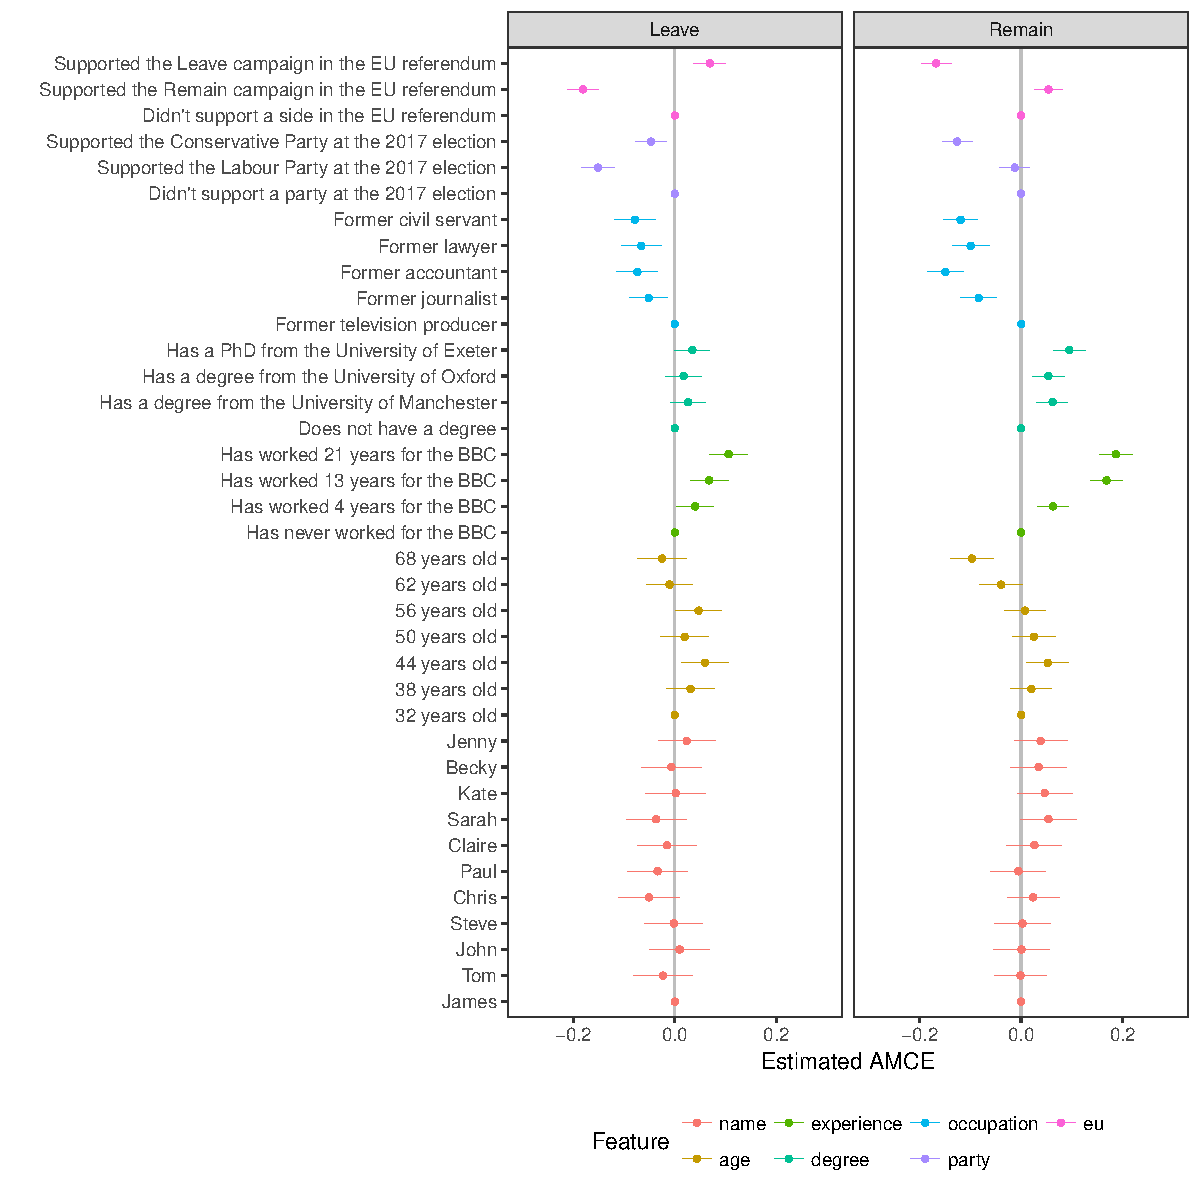
\includegraphics[height=\textheight]{images/conjoint-bbc-1}
\end{center}
}

\frame{
\begin{center}
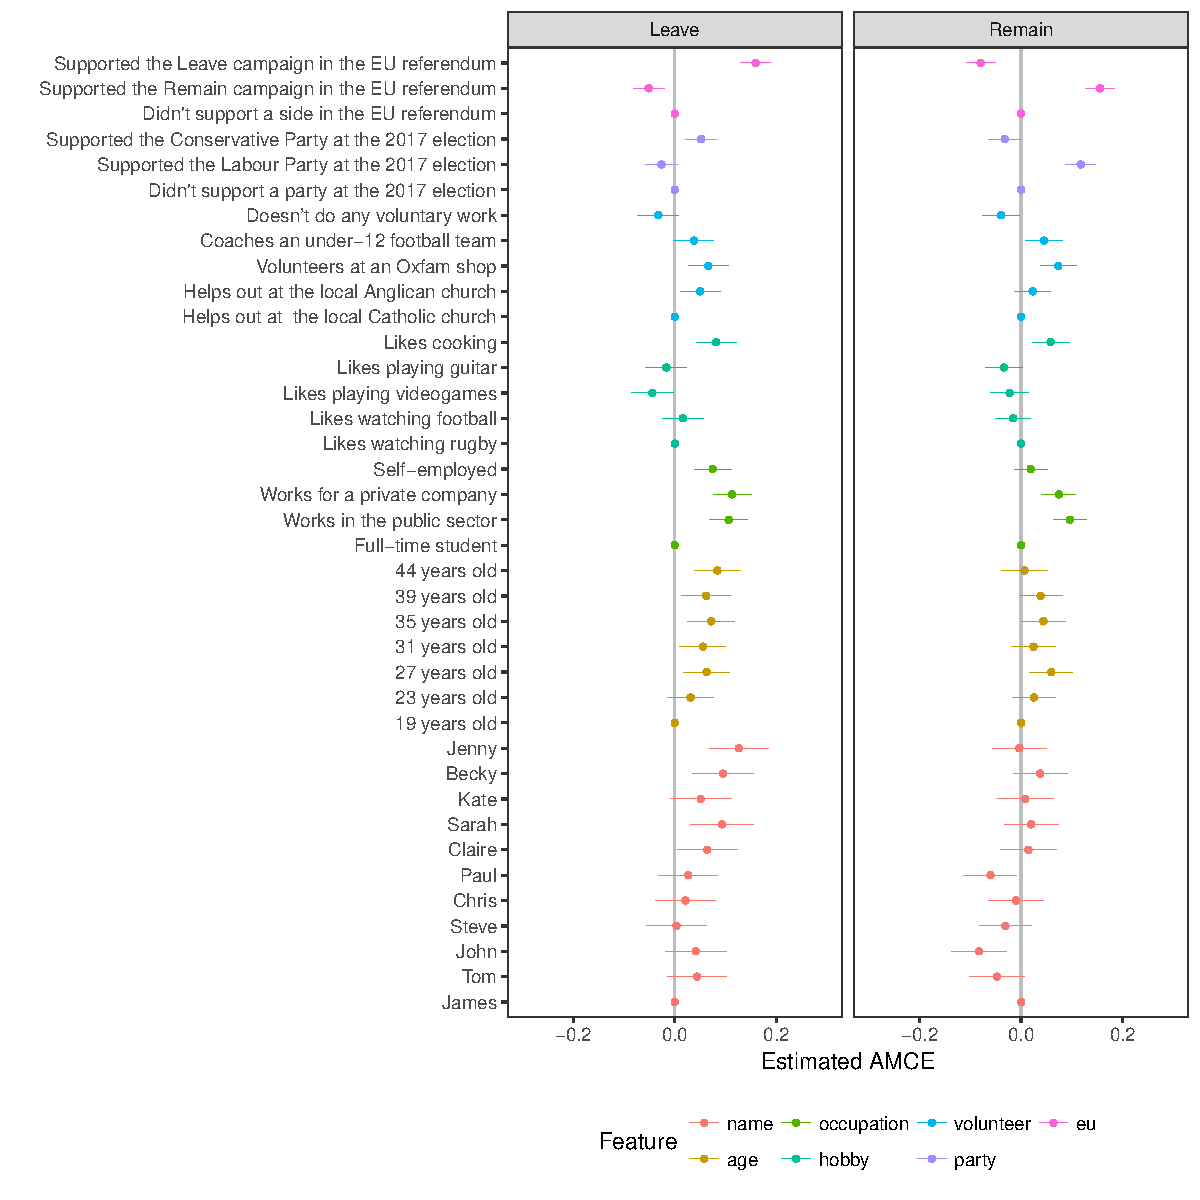
\includegraphics[width=\textheight]{images/conjoint-lodger-1}
\end{center}
}


\frame{

\frametitle{Implementing a Conjoint}

\begin{itemize}\itemsep1em
\item Hope someone else can do it for you!

	\begin{itemize}
	\item Requires programming
	\item Not possible to manually create all possible combinations
	\end{itemize}

\item Strezhnev et al.'s tool:\\
{\small \url{https://scholar.harvard.edu/astrezhnev/conjoint-survey-design-tool}}

\item Qualtrics using Javascript:\\
{\small \url{https://github.com/leeper/conjoint-example}}
\end{itemize}

}


\frame{}


\questions


\frame{

\frametitle{Homework!}

\begin{itemize}\itemsep1em
\item Get a sense of what can be studied survey-experimentally
\item Look at three studies from TESS
	\begin{itemize}\footnotesize
	\item \url{http://tessexperiments.org/data/whillans626.html}
	\item \url{http://tessexperiments.org/data/malhotra634.html}
	\item \url{http://tessexperiments.org/data/nair644.html}
	\end{itemize}
\item We will share them tomorrow
\end{itemize}

}



\appendix
\frame{}

\end{document}
